\documentclass{scrartcl}
\usepackage{etoolbox}
\usepackage{bbm}
\usepackage{amsmath}
\usepackage{mathabx}
\usepackage{graphicx}
\usepackage{float}
\usepackage{parskip}
\usepackage{indentfirst}
\usepackage{subfig}
\usepackage{fancyhdr}
\usepackage{hyperref}
\usepackage[margin=1.25in]{geometry}
\pagestyle{fancy}
\setlength{\parskip}{0em}
\setlength{\parindent}{2em}

%-----------------------------------------------------------------------------
\begin{document}





%-----------------------------------------------------------------------------
% header
\lhead{Huwenbo Shi (603-778-363) shihuwenbo@ucla.edu}

% title
\newcommand*{\TitleFont}{
      \usefont{\encodingdefault}{\rmdefault}{b}{n}
      \fontsize{16}{20}
      \selectfont}
\newcommand*{\AuthorFont}{
      \usefont{\encodingdefault}{\rmdefault}{r}{n}
      \fontsize{12}{20}
      \selectfont}
\title{\TitleFont SoCal: supervised genotype calling via ellipsoidal
separation for Affymetrix SNP microarray}
\author{\AuthorFont Huwenbo Shi (603-778-363) shihuwenbo@ucla.edu}
\date{}
\maketitle
%-----------------------------------------------------------------------------





%-----------------------------------------------------------------------------
% abstract
\begin{abstract}

\centerline{Abstract}

\vspace*{\baselineskip}

\par
\noindent
\textbf{Background:} Genotype calling for SNP microarray is an important
step in array-based association studies.
Most supervised genotype calling methods for SNP microarray fit
generative models (e.g. Gaussian models) on log-transformed allele intensities
of SNPs from samples having reference genotype calls.

\par
\noindent
\textbf{Methods:} In this article, I present SoCal, a supervised genotype
calling method that efficiently finds ellipsoidal decision regions for each
genotype via ellipsoidal separation instead of fitting a generative model.
By assigning different weights to the criteria of finding separating
ellipsoids, SoCal can control the effect of outliers in training data.

\par
\noindent
\textbf{Results:} In leave-one-out cross-validation with HapMap reference
calls, SoCal achieved a concordance rate of 98.94\% at a call rate of 100\%
and 99.71\% at a call rate of 95\%, comparable to many
state-of-the-art methods.
After being trained using HapMap reference calls, SoCal achieved a concordance
rate of 95.10\% with genotype calls made by CRLMM at a call rate of
100\% on a set of validation calls excluding the training calls.
SoCal also shows more robustness than RLMM, a supervised method that uses
Gaussian decision regions to call genotypes, when outliers are present in
training data.
Overall, SoCal is a novel and promising genotype calling method.

\end{abstract}
%-----------------------------------------------------------------------------





%-----------------------------------------------------------------------------
% introduction
\section{Introduction}

\par
% broad background
Accurate genotyping of SNPs is essential to discovering true causal variants
in association studies \cite{gordon2005}.
Although next generation sequencing technology provides cheap whole-genome
sequences for genotyping SNPs, SNP microarray is still a cost-effective
genotyping technology for many specific association studies \cite{rho2010}.
In an Affymetrix SNP microarray, oligonucleotide probes are used to match and
bind DNA fragments containing biallelic SNPs.
Then a fluorescence scanner scans the microarray to quantify perfect 
match and mismatch for these fragments.
Most genotype calling procedures for Affymetrix SNP microarray consist of
two steps.
In the first step, raw information from microarray is summarized to obtain
the intensities, $\theta_A$ and $\theta_B$, of the two alleles, denoted
by A and B, of each SNP.
In the second step, SNPs are classified into genotype AA, AB, or BB based on
the allele intensities they generate.
The focus of this article is on the second step of the genotype calling
procedure---genotype calling using summarized allele intensities.

\par
% specific background
For a specific SNP, if a sample has genotype AA or BB, the allele intensity,
$\theta_A$ or $\theta_B$, will be higher respectively. 
If a sample has genotype AB, the intensities, $\theta_A$ and $\theta_B$,
will be similar.
If one plots $log(\theta_A)$ versus $log(\theta_B)$ of a SNP for a number of
samples, normally 3 ellipsoidal clusters can be observed, one for each
genotype, as shown in Figure~\ref{fig:intro_genclus}.
% state the problem
Many genotype calling algorithms use model-based unsupervised clustering
to identify these clusters and then assign genotypes to each cluster 
\cite{norlen2008,lin2008,fujisawa2004}.
Although these methods are applicable to a wide range of microarrays because
they only require information from microarrays, they don't take advantage of
genotype calls that are already available.
Also, these methods use EM algorithm to estimate model parameters, which is
sensitive to starting parameters and slow to converge \cite{wu1983}.
To utilize reference genotype calls, Rabbee and Speed proposed the RLMM
algorithm, a supervised genotype calling method that forms
decision regions for each genotype by fitting bivariate Gaussian
distributions on log-transformed allele intensities with reference
genotype calls \cite{rabbee2005}.
These Gaussian decision regions are then used to call SNPs for samples with
unknown genotypes.
However, fitting a Gaussian distribution is known to be non-robust to outliers 
\cite{huber1981}.
And for SNP microarrays, outliers can be caused by genomic structural
variations \cite{marioni2007}.

% intro genotype cluster figure
\begin{figure}[H]
\centering
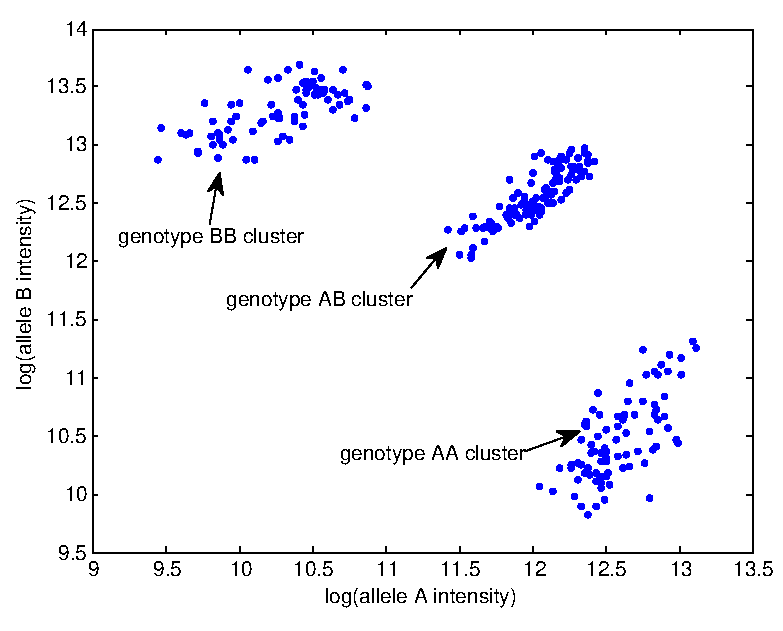
\includegraphics[scale=0.75]{intro_figs/intro_genotype_clusters.pdf}
\caption{Genotype clusters obtained by plotting log-transformed allele
intensities of the two alleles of a SNP for a number of samples.
Each point in the plot represents a sample.}
\label{fig:intro_genclus}
\end{figure}

\par
% state my solution
In this article, I present SoCal, a supervised genotype calling method
for Affymetrix SNP microarray.
Instead of fitting Gaussian distributions on log-transformed allele
intensities with reference genotype calls, SoCal efficiently finds ellipsoidal
decision regions for each genotype via ellipsoidal separation by solving a
conic programming problem.
SoCal can control the effect of outliers by assigning different weights to 
the criteria of finding separating ellipsoids---separation ratio, ellipsoid
volume, and inclusion of points. 
After SoCal finds the ellipsoidal decision regions for each genotype, it uses
them to call SNPs for samples with unknown genotypes using minimum distance
classification.

\par
% state the result
Using reference genotype calls from the HapMap Project as training and
validation data, SoCal achieved a concordance rate of 98.94\% at a call rate
of 100\% and 99.71\% at a call rate of 95\% in leave-one-out
cross-validation.
Furthermore, SoCal showed more robustness than the RLMM method when outliers
were present in training data.
%-----------------------------------------------------------------------------





%-----------------------------------------------------------------------------
% method
\section{Methods}

% overview of method
\subsection{Overview of SoCal's genotype calling procedure}

\par
SNP allele intensities are first normalized and summarized from raw microarray
data using the RMA method, an important preprocessing step that reduces
cross-chip and cross-lab non-biological effects from raw data
\cite{bolstad2003,carvalho2007}.
After the preprocessing step, SoCal calls genotypes in two steps.
In the first step, SoCal finds ellipsoidal decision regions for each genotype
of a SNP using reference genotype calls.
In the second step, SoCal uses these ellipsoidal decision regions to call SNPs
for samples with unknown genotypes through minimum distance classification.

\par
In this section, I first introduce the problem of pattern separation by
ellipsoid.
Then I describe how SoCal finds ellipsoidal decision regions for each
genotype and then calls genotypes using these ellipsoidal decision regions.

% pattern separation via ellipsoids
\subsection{Pattern separation by ellipsoid}

\par
An ellipsoid $\mathcal{E} \subseteq \mathbbm{R}^{n}$ can be expressed as
$\mathcal{E} = \{x \in \mathbbm{R}^{n} | (x-c)^TE(x-c)\leqslant1\}$, where
$c$ is the center of the ellipsoid, and $E$ a positive definite matrix
denoting the shape and orientation of the ellipsoid.
Let $\{a_i\}$ be the points to be included in an ellipsoid, and $\{b_j\}$
be the points to be excluded, the problem of ellipsoidal separation is to find
$c$ and $E$ such that $(a_i-c)^TE(a_i-c)\leqslant1 \, \forall i$ and
$(b_j-c)^TE(b_j-c)>1 \, \forall j$.

% ellipsoidal pattern separation formulation
\subsection{Forming ellipsoidal decision regions for each genotype}

\par
Let $G=\{AA,AB,BB\}$ be the set of genotypes of SNP $n$, and $J_{AA}$,
$J_{AB}$, $J_{BB}$ the index set of samples with the corresponding genotype.
Let $X=\{(log(\theta_A),log(\theta_B))_i|i=1,\cdots,
|J_{AA}|+|J_{AB}|+|J_{BB}|\}$ be the set of log-transformed allele intensities
of all the samples, and $X_{AA}=\{x_j|x_j \in X, j \in J_{AA}\}$,
$X_{AB}=\{x_j|x_j \in X, j \in J_{AB}\}$,
$X_{BB}=\{x_j|x_j \in X, j \in J_{BB}\}$ the set of log-transformed allele
intensities from samples having the corresponding genotype for SNP $n$.

\par
To find the ellipsoid that includes $X_{AA}$ and excludes
$X_{AB} \cup X_{BB}$, one
sets $\{a_i\}=X_{AA}$ and $\{b_j\}=X_{AB} \cup X_{BB}$, and
solves the following conic programming problem.
\begin{equation*}
\begin{aligned}
& \text{minimize}
&& -{\beta_{1}}k+{\beta_{2}} trace(T)+\beta_{3} \|u-\mathbbm{1}\|_1 \\  
& \text{subject to}
&& (1,a_i)^T\tilde{E}(1,a_i)\leqslant u_i \; \forall i \\
&&&(1,b_j)^T\tilde{E}(1,b_j) \ge k \; \forall j \\
&&&\tilde{E}=
    \left[
        \begin{array}{cc}
            s & v^T \\
            v & F
        \end{array}
    \right] \succeq 0 \\
&&&\left[
        \begin{array}{cc}
            F & I \\
            I & T
        \end{array}
    \right] \succeq 0
\end{aligned}
\end{equation*}

\par
Here, $I$ denotes the identity matrix.
Derivation of the problem formulation is largely followed from
\cite{glineur1998}.
For the sake of space, detailed derivation of the problem formulation is not
presented here.
In the problem formulation above, $\beta_{i} > 0$ are the weights assigned to
the criteria of finding separating ellipsoid---separation ratio,
ellipsoid volume, and inclusion of points.
By increasing $\beta_2$, one finds ellipsoid with
smaller volume.
And by increasing $\beta_3$, one finds ellipsoid that tries to
include more data points.
In SoCal, default values for $\beta_1$, $\beta_2$, $\beta_3$ are
empirically set to 1, $10^4$, and $10^2$ respectively.

\par
Let 
$\tilde{E}^{*}=\left[
    \begin{array}{cc}
    s & v^T \\
    v & F
    \end{array}
\right]$
be the optimal solution to the problem above.
The separating ellipsoid $\mathcal{E}^{*}$ is defined as
$\mathcal{E}^{*}=
\{x \in \mathbbm{R}^{n}|(x-c^{*})^TE^{*}(x-c^{*})\leqslant2(1+k)\}$,
where $c^{*}=-F^{-1}v,\;E^{*}={{F} \over {(1-s+{c^{*}}^TF{c^{*}})}}$.

\par
To find the ellipsoid that includes $X_{AB}$ and excludes
$X_{AA} \cup X_{BB}$, one sets $\{a_i\}=X_{AB}$ and
$\{b_j\}=X_{AA} \cup X_{BB}$, and solves the above conic programming problem.
The same procedure also applies to finding the ellipsoid that includes $X_{BB}$
and excludes $X_{AA} \cup X_{AB}$.

% handling missing clusters
\subsection{Handling sparse or missing genotype clusters}
\par
If a SNP has moderate minor allele frequency (MAF), the genotype clusters of
that SNP are well defined, and SoCal obtains three ellipsoidal decision
regions for that SNP, one for each genotype cluster
(Figure \ref{fig:defined_cluster}).
However, if a SNP has lower MAF, some genotype cluster may be sparse
or missing.
For these SNPs, SoCal estimates the ellipsoid for the sparse or missing
genotype cluster using the ellipsoids for the other two genotypes through
simple geometric transformations (Figure \ref{fig:sparse_cluster}).

\begin{figure}[H]
    \centering
    \subfloat[SNP with 3 well defined genotype clusters.
              SoCal obtains one ellipsoid for each genotype cluster.] {
        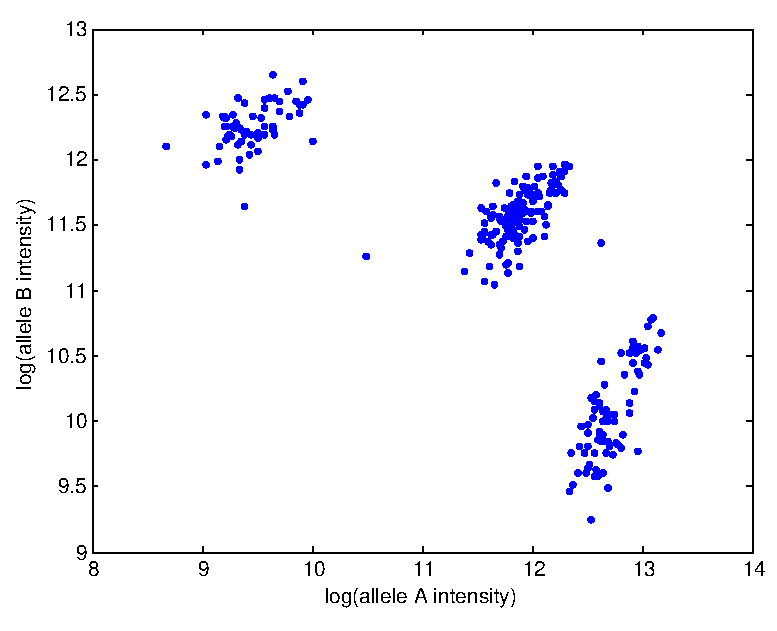
\includegraphics[scale=0.5]{method_figs/defined_cluster.pdf}
        \label{fig:defined_cluster}
    }
    \qquad
    \subfloat[SNP with sparse genotype BB cluster.
              SoCal first obtains ellipsoids for genotype AA and AB clusters,
              and then estimates the ellipsoid (drawn in dashed line) for
              genotype BB cluster.] {
        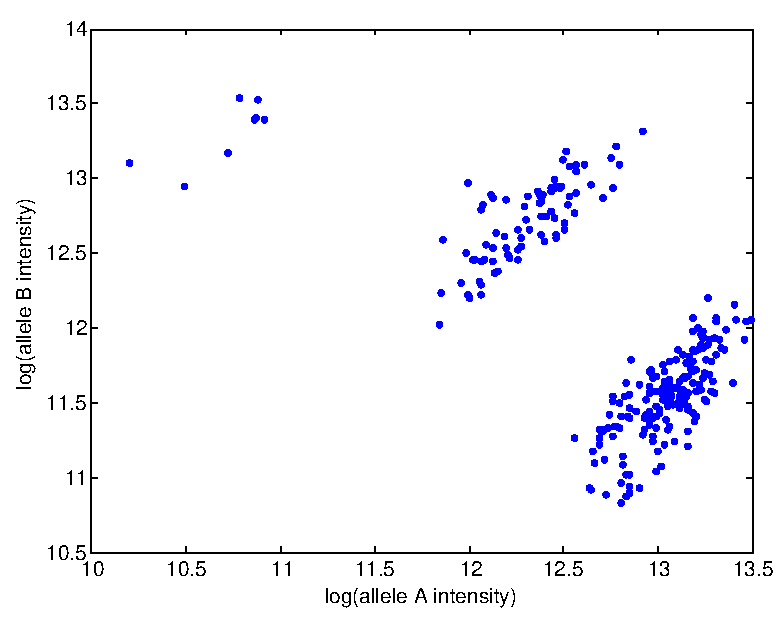
\includegraphics[scale=0.5]{method_figs/sparse_cluster.pdf}
        \label{fig:sparse_cluster}
    }
    \caption{Ellipsoids obtained by SoCal for SNPs with well-defined and
             sparse genotype clusters.
             Each dot in the plots represents a sample, with samples having
             HapMap reference genotype calls marked as red triangles.
             The ellipsoids are obtained using all the reference calls.}
             
    \label{fig:defined_sparse_cluster}
\end{figure}

% missing genotype aa cluster
\subsubsection{Missing genotype AA or BB cluster}

\par
If genotype AA cluster of a SNP has less than 3 reference calls, SoCal
first finds the ellipsoids for genotype AB and BB clusters, and then
estimates that for genotype AA cluster through simple geometric
transformations.

\par
Let $\mathcal{E}_{AB}=
\{x \in \mathbbm{R}^{n}|(x-c_{AB})^TE_{AB}(x-c_{AB}) \leqslant 1\}$
and $\mathcal{E}_{BB}=
\{x \in \mathbbm{R}^{n}|(x-c_{BB})^TE_{BB}(x-c_{BB}) \leqslant 1\}$
be the ellipsoids obtained for genotype AB and BB clusters,
and $n_{AB}$, $n_{BB}$ the unit vectors pointing in the direction of
the major axis of the corresponding ellipsoid.
SoCal estimates the center of $\mathcal{E}_{AA}$, the ellipsoid for genotype
AA cluster, by reflecting $c_{BB}$, the center of $\mathcal{E}_{BB}$, across
the major axis of $\mathcal{E}_{AB}$.
To estimate the orientation of $\mathcal{E}_{AA}$, SoCal first determines the
angle between $n_{AB}$ and $n_{BB}$, and then applies a rotation matrix of
that angle on $E_{AB}$.

\par
Formally, let $\mathcal{E}_{AA}=
\{x \in \mathbbm{R}^{n}|(x-c_{AA})^TE_{AA}(x-c_{AA}) \leqslant 1\}$ be the
estimated ellipsoid for genotype AA cluster, and $\alpha$ the angle between
$n_{AB}$ and $n_{BB}$, then
$c_{AA}=-c_{BB}+2c_{AB}+2n_{AB}((c_{BB}-c_{AB})^{T}n_{AB})$, and
$E_{AA}=R^{T}E_{AB}R$, where $R$ is a rotation matrix of angle $\alpha$.

\par
If genotype BB cluster is missing, the center and orientation of the
ellipsoid for that cluster is estimated in a similar way.
Formally, let $\mathcal{E}_{BB}=
\{x \in \mathbbm{R}^{n}|(x-c_{BB})^TE_{BB}(x-c_{BB}) \leqslant 1\}$ be the
estimated ellipsoid for genotype BB cluster, and $\alpha$ the angle between
$n_{AB}$ and $n_{AA}$, then
$c_{BB}=-c_{AA}+2c_{AB}+2n_{AB}((c_{AA}-c_{AB})^{T}n_{AB})$, and
$E_{BB}=R^{T}E_{AB}R$, where $R$ is a rotation matrix of angle $-\alpha$.

% missing genotype ab cluster
\subsubsection{Missing genotype AB cluster}

Although SNPs with genotype AB cluster missing were not observed in HapMap
reference genotype calls, for completeness, for these SNPs SoCal first
obtains, $\mathcal{E}_{AA}$ and $\mathcal{E}_{BB}$,
the ellipsoids for genotype AA and BB cluster, and then estimates the
center of $\mathcal{E}_{AB}$, the ellipsoid for the missing cluster, using
the mid-point between the centers of $\mathcal{E}_{AA}$ and $\mathcal{E}_{BB}$.
The orientation of $\mathcal{E}_{AB}$ is obtained by applying a rotation
to the ellipsoid with the minimum volume among $\mathcal{E}_{AA}$ and
$\mathcal{E}_{BB}$.

\par
Formally, let $\mathcal{E}_{AB}=
\{x \in \mathbbm{R}^{n}|(x-c_{AB})^TE_{AB}(x-c_{AB}) \leqslant 1\}$ be the
estimated ellipsoid for genotype AB cluster, and $\alpha$ the angle between
$n_{AA}$ and $n_{BB}$, then
$c_{AB}=(c_{AA}+c_{BB})/2$, and
$E_{AB}=R^{T}\hat{E}R$, where $\hat{E}$ is the matrix of the ellipsoid
with the minimum volumne among $\mathcal{E}_{AA}$ and $\mathcal{E}_{BB}$, and
$R$ a rotation matrix of angle $\pm\alpha/2$.
The sign of the angle of rotation is dependent on the choise of ellipsoid on
which rotation is applied---positive for $\mathcal{E}_{AA}$ and negative
for $\mathcal{E}_{BB}$.

% genotype calling
\subsection{Genotype calling}

\par
After the ellipsoidal decision regions,
$\mathcal{E}_{g}=
\{x \in \mathbbm{R}^{n} | (x-c_g)^TE_g(x-c_g) \leqslant 1\},
\forall g\in\{AA,AB,BB\}$ of a SNP are obtained, SoCal uses them to classify
SNPs for samples with unknown genotypes using minimum distance classification.

\par
If a sample has allele intensities $\theta_A$ and $\theta_B$ at SNP $n$,
SoCal first computes
$D_g=\sqrt{(x-c_g)^TE_g(x-c_g)}$,
where $x=(log(\theta_A), log(\theta_B))$, for each $g\in\{AA,AB,BB\}$.
SoCal then calls the genotype, $\mathcal{G}$, of that sample at SNP $n$
as the genotype having minimum $D_g$, that is,
$\mathcal{G}=\operatorname*{arg\,min}_{g\in \{AA,AB,BB\}}D_g$.

\par
SoCal defines $\lambda=1-D_{\mathcal{G}}/(D_{AA}+D_{AB}+D_{BB})$ to quantify
the confidence of each genotype call.
By increasing the threshold for $\lambda$, SoCal can achieve higher call
accuracy at the cost of decreasing call rate.
%-----------------------------------------------------------------------------





%-----------------------------------------------------------------------------
% data
\section{Materials}

\par
The microarray used for evaluation in this project was the Affymetrix GeneChip
Human Mapping 50K Xba Array, which contains 58,960 SNPs.
Raw microarray data for 270 samples was obtained from HapMap FTP, and
reference genotype calls were obtained from HapMap using
HapMart \cite{hapmap2003}.

\par
After removing strand-ambiguous SNPs and SNPs not present on HapMart from the
set of SNPs on the microarry, 16,387 SNPs were left.
Figure~\ref{fig:data_maf_dist} shows the minor allele frequency distribution
for these SNPs.

% maf distribution figure
\begin{figure}[H]
\centering
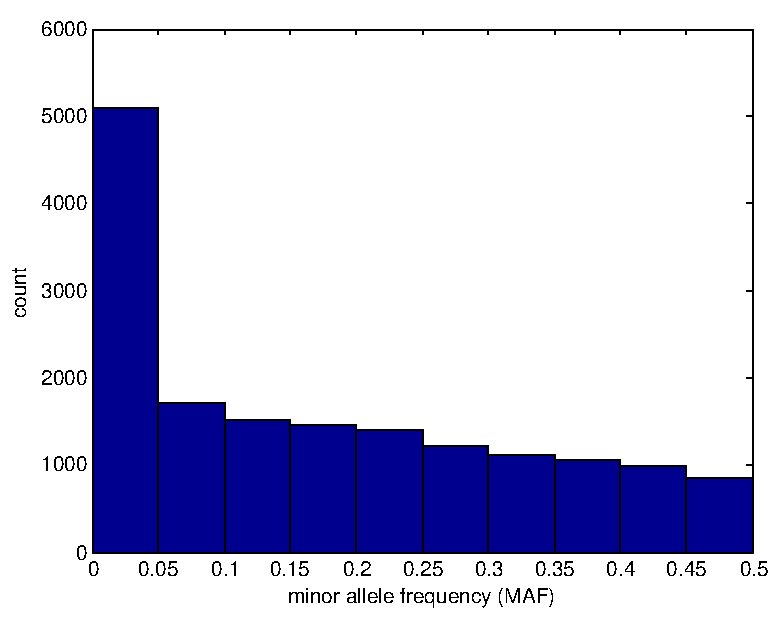
\includegraphics[scale=0.75]
{data_figs/maf_dist.pdf}
\caption{Minor allele frequency distribution for the 16,387 SNPs.}
\label{fig:data_maf_dist}
\end{figure}

\par
From the 16,387 SNPs, 4,064 SNPs with two genotype clusters having less than
3 reference genotype calls were further removed.
Among these SNPs, 3,596 are monomorphic SNPs with MAF equal to 0.
In total, 12,323 SNPs were left for evaluation.
On average, each of these SNPs has 83 reference genotype calls.
%-----------------------------------------------------------------------------





%-----------------------------------------------------------------------------
% result
\section{Results}

% result for comparing socal with hapmap calls
\subsection{Cross-validation with HapMap reference calls}

\par
To evaluate the accuracy of SoCal, I compared the genotype calls made by SoCal
with the reference calls from HapMap through leave-one-out
cross-validation.
For each SNP, I used one sample from the reference set as validation data and
the rest as training data.
I repeated this process until all the samples in the reference set were used
as validation data exactly once.
Concordance rate is defined as the ratio between the number of calls that are
concordant with HapMap reference calls and the total number of calls made by
SoCal.

\par
First, I compared the accuracy of SoCal under different choices of $\beta_i$,
the weights assigned to the criteria of finding ellipsoidal decision regions
for each genotype cluster.
Figure~\ref{fig:result_sh_crvacc} shows the concordance rate of SoCal in the
leave-one-out cross-validation at a wide range of call rates for different
values of $\beta_i$.
Because the weights, $\beta_1=1$, $\beta_2=10^4$, $\beta_3=10^2$,
had the highest call rates at fixed concordance rates, they are set to be the
default of SoCal.
And all other experiments presented in this article used this choice
of weights.

% accuracy as function of call rate
\begin{figure}[H]
\centering
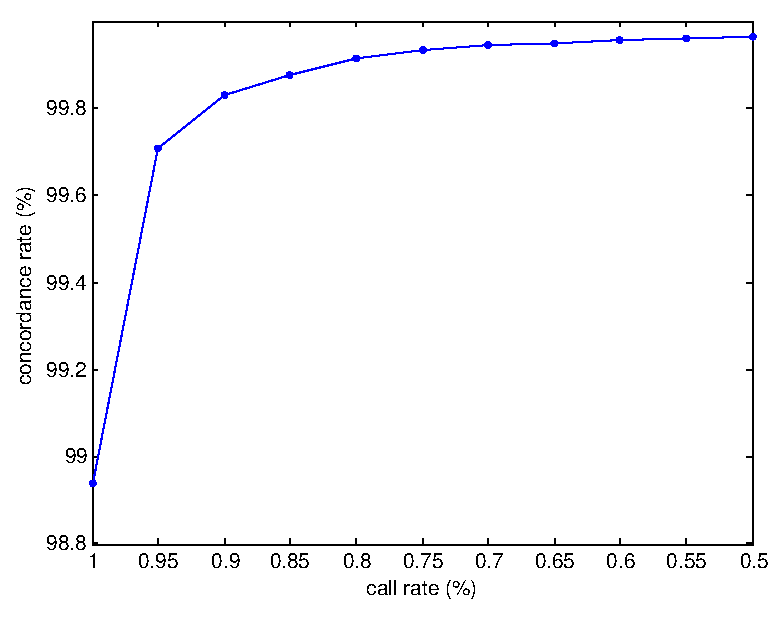
\includegraphics[scale=0.75]
{result_figs/cmp_socal_hapmap/cmp_socal_hapmap_cr_vs_acc.pdf}
\caption{Concordance rate of SoCal in the leave-one-out cross-validation with
HapMap reference calls as a function of call rate, for different choices of
$\beta_i$}
\label{fig:result_sh_crvacc}
\end{figure}

\par
Table~\ref{table:cmp_hapmap_socal_100} shows the genotype calls made by SoCal
and the reference calls from HapMap in leave-one-out cross-validation.
At a call rate of 100\%, SoCal made 1,081,319 calls in total, out of which
1,069,857 were concordant with HapMap calls, achieving a concordance
rate of 98.94\%.

% 100% call rate result
\begin{table}[H]
\centering
\begin{tabular}{l*{5}{r}r}
    \hline
    HapMap/SoCal  & AA       & AB      & BB      & No Call \\ \hline
    AA            & 360,289  & 2,282   & 1,058   & 0  \\
    AB            & 2,667    & 341,012 & 2,257   & 0  \\
    BB            & 851      & 2,347   & 368,556 & 0  \\ \hline
\end{tabular}
\caption{At a call rate of 100\%, SoCal achieved 98.94\% concordance rate
in leave-one-out cross-validation with HapMap reference calls.}
\label{table:cmp_hapmap_socal_100}
\end{table}

\par
Table~\ref{table:cmp_hapmap_socal_95} shows detailed comparison between
SoCal and HapMap calls at a call rate of 95\%.
At a call rate of 95\%, SoCal made 1,028,258 calls in total, out of which
1,025,242 were concordant with HapMap calls, achieving a concordance
rate of 99.71\%.
These results are comparable to those achieved by previous methods
\cite{rabbee2005,di2005}.

% 95% call rate result
\begin{table}[H]
\centering
\begin{tabular}{l*{5}{r}r}
    \hline
    HapMap/SoCal  & AA       & AB      & BB      & No Call \\ \hline
    AA            & 348,221  & 390     & 298     & 14,720  \\
    AB            & 710      & 319,394 & 775     & 25,057  \\
    BB            & 410      & 427     & 357,627 & 13,290  \\ \hline
\end{tabular}
\caption{At a call rate of 95\%, SoCal achieved 99.71\% concordance rate
in leave-one-out cross-validation with HapMap reference calls.}
\label{table:cmp_hapmap_socal_95}
\end{table}

% comparison with crlmm
\subsection{Comparison with CRLMM calls}

\par
As another way of evaluating the accuracy of SoCal, I compared the genotype
calls made by SoCal and those made by CRLMM, a state-of-the-art
supervised genotype calling method for SNP microarrays that uses a two-level
hierarchical model to model variations in allele intensities
across SNPs and across chips \cite{carvalho2007}.

\par
I first trained SoCal using all the samples with HapMap reference calls, and
then made genotype calls on the rest of the samples.
When comparing SoCal with CRLMM, I excluded the training samples and compared
these two methods only at samples not in the training set.

\par
Table~\ref{table:cmp_socal_crlmm} shows detailed comparison between SoCal
and CRLMM at a call rate of 100\%.
In total, SoCal made 2,245,891 calls, out of which 2,134,868 were concordant
with those made by CRLMM, achieving a concordance rate of 95.10\%.
The high concordance rate between SoCal and CRLMM suggests that genotype
calling via ellipsoidal separation instead of fitting generative models
is a promising approach.

% detail comparison between socal and crlmm
\begin{table}[H]
\centering
\begin{tabular}{l*{5}{r}r}
    \hline
    CRLMM/SoCal   & AA       & AB      & BB      & No Call \\ \hline
    AA            & 781,903  & 23,244  & 10,405  & 0  \\
    AB            & 22,340   & 564,280 & 22,533  & 0  \\
    BB            & 7,730    & 24,771  & 788,685 & 0  \\ \hline
\end{tabular}
\caption{At a call rate of 100\%, SoCal achieved 95.10\% concordance rate
with the calls made by CRLMM. Training samples for SoCal were excluded during
comparison.}
\label{table:cmp_socal_crlmm}
\end{table}

% comparison with rlmm
\subsection{Comparison with RLMM in the presence of outliers}

\par
I investigated how robust SoCal is when outliers are present in training data.
For comparison, I implemented the RLMM algorithm, which fits bivariate
Gaussian distributions on log-transformed allele intensities
of each genotype cluster and then classifies SNPs with unknown genotype into
the distribution having minimum Mahalanobis distance based on the allele
intensities they generate \cite{rabbee2005}.

\par
For accurate comparison, I selected a subset of 3,442 SNPs that have
more than 10 reference calls for each genotype cluster from the set of
12,323 SNPs used for evaluation in previous experiments.
To simulate outliers, for each SNP, I first estimated $\mu_g$, the mean of
log-transformed allele intensities of each genotype cluster, and then
drew one outlier for each genotype cluster from the Gaussian distribution
$N(\mu_g, \gamma I)$, where $I$ is the identity matrix and $\gamma$ a
positive constant controlling the variance of the distribution---by increasing
$\gamma$, one increases the effect of outliers.
In total, I simulated 3 outliers for each SNP, one for each genotype cluster.

\par
To illustrate the robustness of SoCal and RLMM,
Figure~\ref{fig:cmp_shape_noise} shows the ellipsoidal decision
regions obtained by SoCal and the level curves of the Gaussian decision regions
obtained by RLMM before and after an outlier is introduced to the genotype AA
cluster.
Before an outlier is introduced, both SoCal and RLMM can find appropriate
decision regions for each genotype cluster and make accurate genotype calls.
However, after an outlier is introduced into the genotype AA cluster, the
estimated variance of the Gaussian decision region obtained by RLMM for the
genotype AA cluster is significantly affected, making genotype calling much
less accurate.
On the other hand, because SoCal not only considers outliers but also
jointly uses data points from other genotype clusters when forming the decision
regions, the decision region for the genotype AA cluster, although affected, is
still accurate enough to classify all samples into correct genotypes.

% figure to illustrate socal vs gauss in terms of noise
\begin{figure}[H]
    \centering
    \subfloat[Decision regions formed by SoCal when there is no outlier.] {
        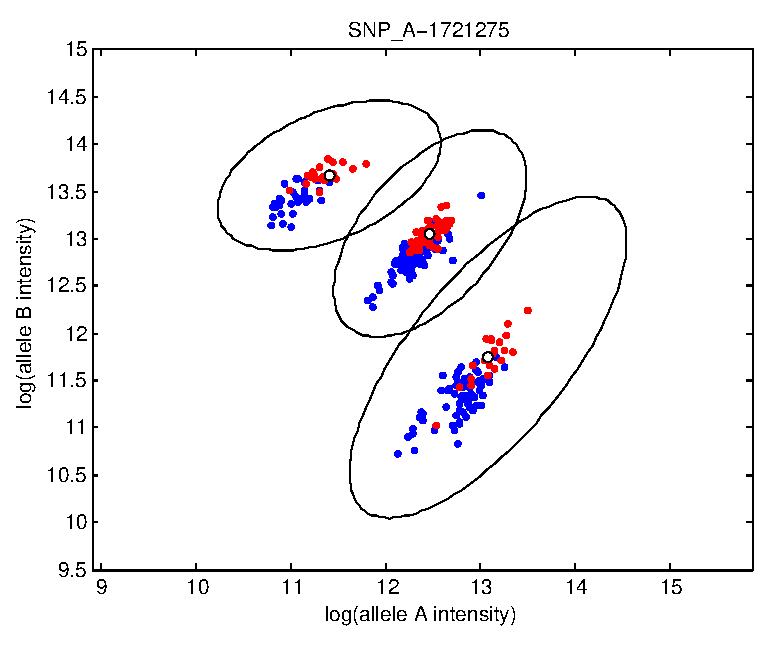
\includegraphics[scale=0.5]
            {result_figs/cmp_socal_gauss_noise_shape/ellipse_no_noise.pdf}
        \label{fig:socal_region_no_noise}
    }
    \qquad
    \subfloat[Decision regions formed by RLMM when there is no outlier.] {
        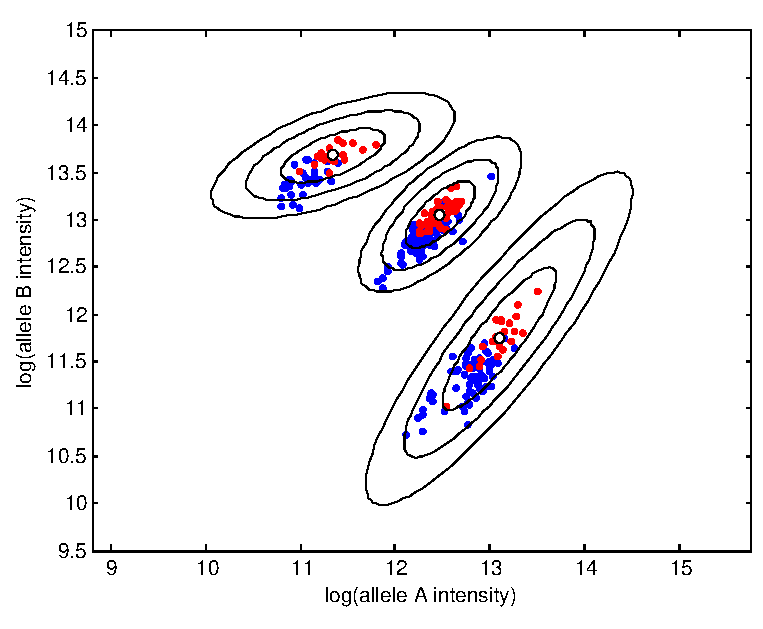
\includegraphics[scale=0.5]
            {result_figs/cmp_socal_gauss_noise_shape/gauss_no_noise.pdf}
        \label{fig:gauss_region_no_noise}
    }
    \\
    \subfloat[Decision regions formed by SoCal when an outlier
              (diamond-shaped point) is introduced into the genotype AA
              cluster.
              Although affected, these decision regions can still classify all
              samples into correct genotypes.] {
        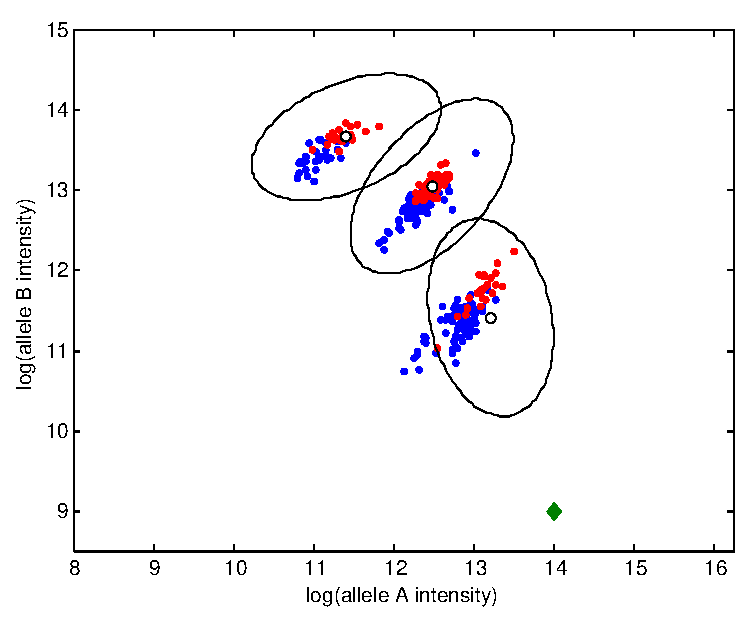
\includegraphics[scale=0.5]
            {result_figs/cmp_socal_gauss_noise_shape/ellipse_noise.pdf}
        \label{fig:socal_region_no_noise}
    }
    \qquad
    \subfloat[Decision regions formed by RLMM when an outlier
              (diamond-shaped point) is introduced into the genotype
              AA cluster.
              The estimated variance of the bivariate Gaussian distribution is
              significantly affected, and RLMM may mistakenly
              classify samples with genotype AB into genotype AA.] {
        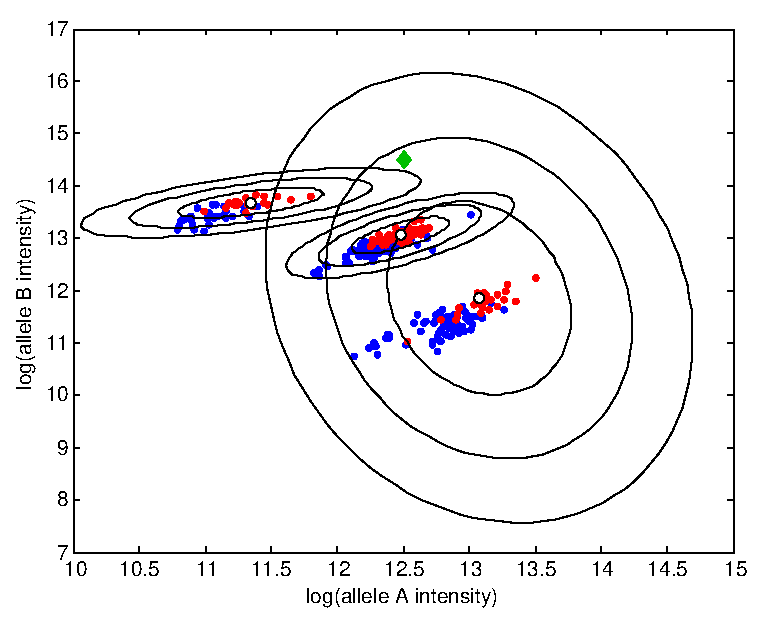
\includegraphics[scale=0.5]
            {result_figs/cmp_socal_gauss_noise_shape/gauss_noise.pdf}
        \label{fig:gauss_region_no_noise}
    }
    \caption{Decision regions formed by SoCal and RLMM before and after an
             outlier is introduced to the genotype AA cluster.
             Samples with reference genotype calls are marked as red
             triangles.}
    \label{fig:cmp_shape_noise}
\end{figure}

\par
Figure~\ref{fig:result_cmp_noise} shows the decrease in concordance rate of
SoCal and RLMM at call rate of 100\% in leave-one-out cross-validation with
HapMap reference genotype calls as the variance of simulated outliers varies
from 1 to 10.
Clearly, the concordance rate of SoCal decreases much more slowly than does
the RLMM method.
Thus, SoCal is in general more robust to outliers than RLMM.

% accuracy as function of noise variance
\begin{figure}[H]
\centering
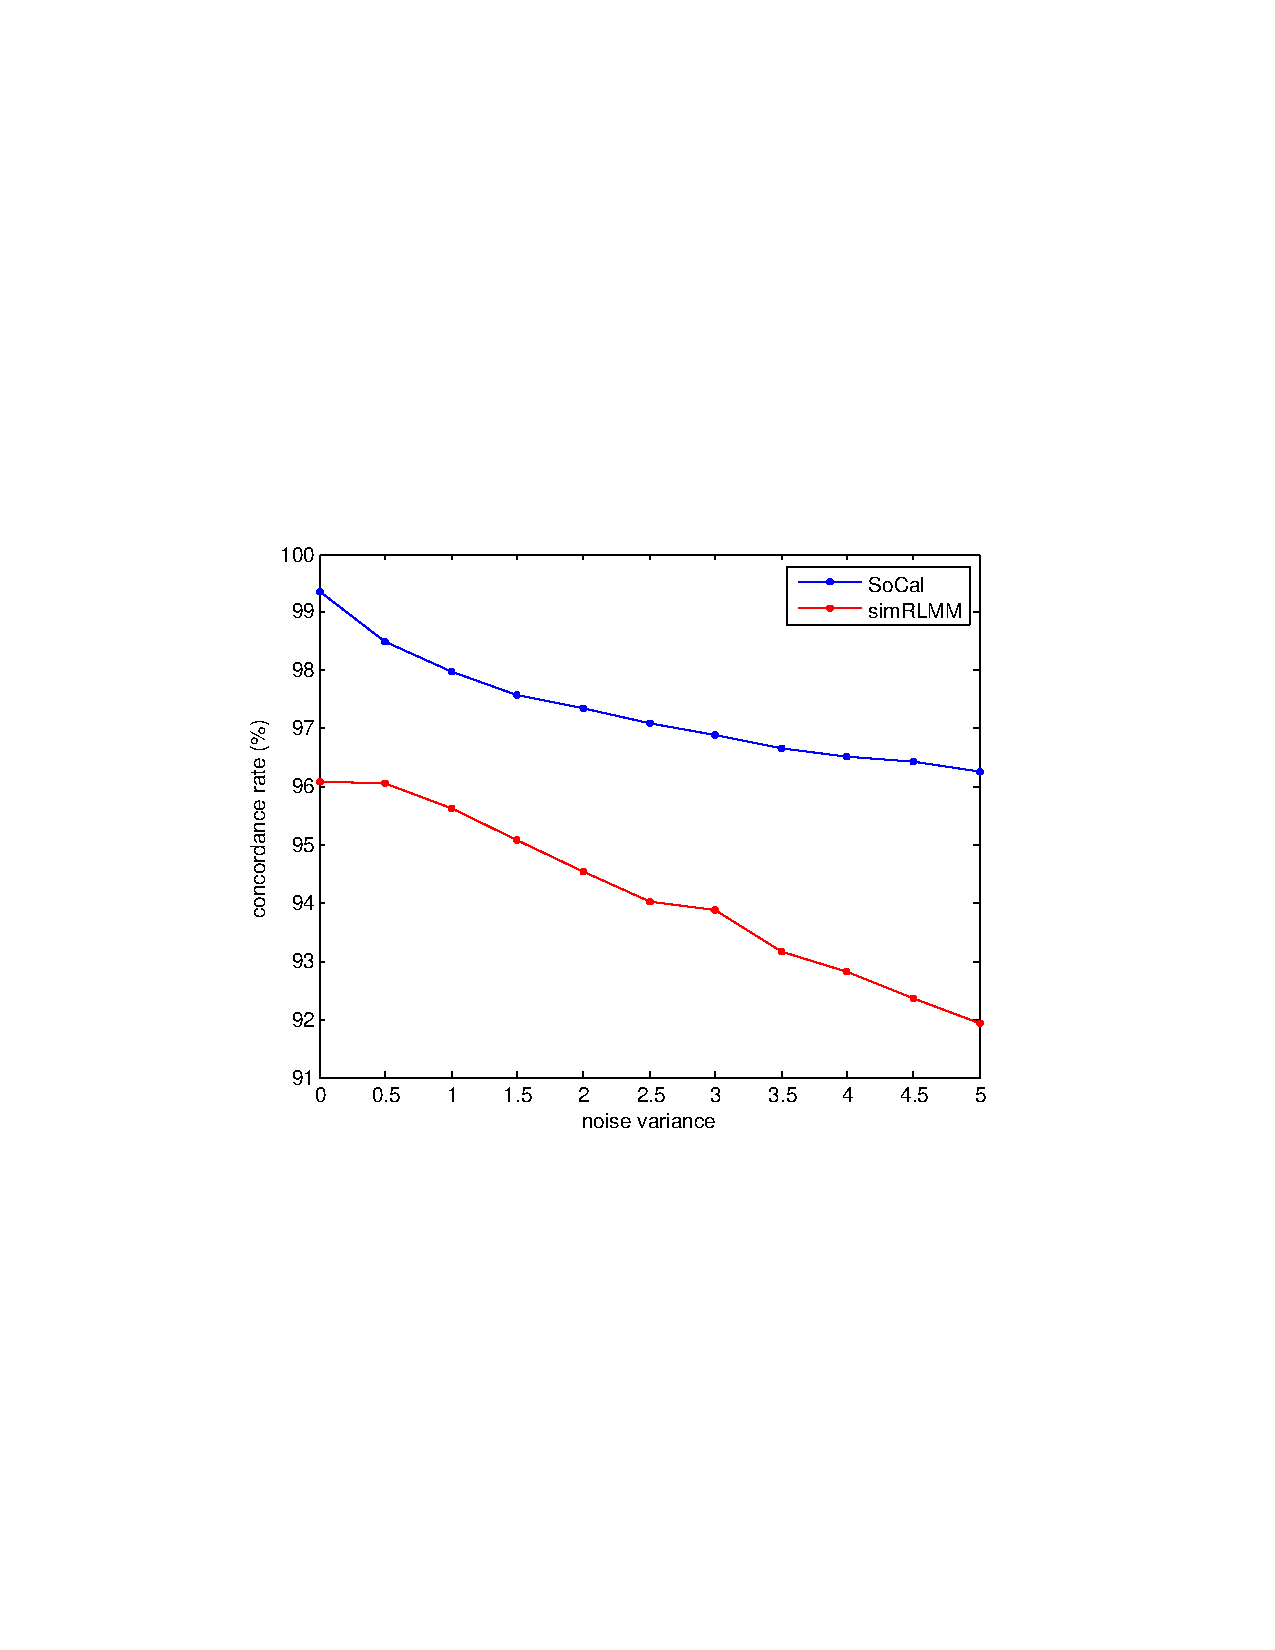
\includegraphics[scale=0.75]
{result_figs/cmp_socal_gauss_noise/socal_gauss_cmp_noise.pdf}
\caption{Concordance rate of SoCal and RLMM in the leave-one-out
cross-validation with HapMap reference calls as a function of outlier
variance.}
\label{fig:result_cmp_noise}
\end{figure}

% implementation
\subsection{Software implementation and running time}

\par
SoCal is implemented in Python.
To solve the conic programming problem of finding separating ellipsoids,
SoCal uses CVXOPT, a Python wrapper for optimization problem solvers written
in C, that can solve conic programming problems in polynomial
time \cite{andersen2014}.
Source code of SoCal is available at
\url{https://github.com/huwenboshi/wqe/tree/master/genotype_caller}.

\par
On average, SoCal takes 0.2 CPU second to obtain ellipsoidal decision
regions for each SNP.
For a SNP microarray that has 100,000 SNPs, SoCal will take approximately
5.56 CPU hours to obtain decision regions for all the SNPs.
This is a reasonable time investment.
And the training process of SoCal is easily parallelizable.
After the decision regions of all the SNPs are obtained, SoCal can call
future SNPs in linear time.
%-----------------------------------------------------------------------------






%-----------------------------------------------------------------------------
% discussion
\section{Discussion}

\par
I have presented SoCal, a supervised genotype calling algorithm for Affymetrix
SNP microarray.
Unlike most existing supervised genotype calling algorithms that try to fit
generative models (e.g. Gaussian models) on log-transformed allele
intensities of SNPs from samples with reference genotype calls,
SoCal uses these data to efficiently finds ellipsoidal decision regions for
each genotype cluster via ellipsoidal separation by solving a conic
programming problem.
Both cross-validation with HapMap reference calls and comparison with
genotype calls made by CRLMM show that SoCal is comparable in accuracy to many
of the state-of-the-art genotype calling methods.
Also, when outliers are present in training data, SoCal outperforms RLMM, a
genotype calling method that uses Gaussian decision regions to call genotypes,
demonstrating the robustness of SoCal over existing methods.
Overall, SoCal is a novel and promising genotype caller for
Affymetrix SNP microarray.

\par
Like many supervised genotype calling methods, SoCal has its limitations.
First, SoCal is not directly applicable to SNPs that don't have
reference genotype calls.
In this case, one can first call genotypes from microarrays using
unsupervised genotype calling methods.
Then one can treat these calls as training data and use SoCal to
form refined ellipsoidal decision regions for each genotype cluster.
Because SoCal is robust to outliers in training data, the refined
ellipsoidal decision regions can be directly used to accurately call genotypes
for future samples.
Another limitation of SoCal is that users need to tune the weights
assigned to the criteria of finding the separating ellipsoids
for different microarrays.
However, experiments with SoCal using different weights show that SoCal is
relatively less sensitive to weight parameters if $\beta_3$, the weight
assigned to the criterion of inclusion of points, is set to $10^2$.

\par
SoCal is still in development, and can be improved and extended in
many directions.
First, the current approach that SoCal uses to handle SNPs with sparse or
missing genotype clusters is through simple and fixed geometric
transformations.
This approach assumes that genotype AA cluster and genotype BB cluster are
symmetric around genotype AB cluster.
However, this is not true in general.
An improvement to this approach is to estimate the positions and orientations
of the ellipsoids for sparse or missing clusters using information from
SNPs with well-defined clusters that generate similar allele
intensities patterns. 
Second, SoCal currently only uses allele intensities data from samples having
reference genotype calls.
However, allele intensities data for samples having structural variations is
also available from the HapMap Project \cite{hapmap2003}.
A possible improvement for SoCal is to include these data in finding the
ellipsoidal decision regions for each genotype cluster to further refine the
decision regions of each genotype.
These refined decision regions can then be used to call genotypes more
accurately and to detect outliers and possible structural variations.

\par
To summarize, SoCal presents a novel and promising method for genotype calling.
It's efficient in that it finds decision regions for each genotype via
ellipsoidal separation by solving a conic programming problem, which is
solvable in polynomial time with guaranteed global optimum \cite{glineur1998}.
Also, SoCal is comparable in accuracy to many state-of-the-art methods.
Although SoCal has the limitation that training data must be available, this
limitation is also present in other supervised genotype calling methods, and
has been addressed previously \cite{carvalho2007}.
Finally, SoCal can also be extended and improved to be more accurate and to
have more functionality.
%-----------------------------------------------------------------------------




%-----------------------------------------------------------------------------
% references
\begin{thebibliography}{9}

\bibitem{gordon2005}
Gordon D, Finch SJ. Factors affecting statistical power in the detection of
genetic association. J Clin Invest. 2005;115(6):1408-18.

\bibitem{rho2010}
Roh SW, Abell GC, Kim KH, Nam YD, Bae JW. Comparing microarrays and
next-generation sequencing technologies for microbial ecology research.
Trends Biotechnol. 2010;28(6):291-9.

\bibitem{norlen2008}
Norl\'{e}n, H., Pettersson, E., Ahmadian, A., Lundeberg, J., \& Sundberg, R.
(2008). Classification of SNP genotypes by a Gaussian mixture model in
competitive enzymatic assays.
Mathematical Statistics Stockholm University Research Report, 3, 1-26.

\bibitem{lin2008}
Lin Y, Tseng GC, Cheong SY, Bean LJ, Sherman SL, Feingold E. Smarter
clustering methods for SNP genotype calling.
Bioinformatics. 2008;24(23):2665-71.

\bibitem{fujisawa2004}
Fujisawa H, Eguchi S, Ushijima M, et al. Genotyping of single nucleotide
polymorphism using model-based clustering. Bioinformatics. 2004;20(5):718-26.

\bibitem{wu1983}
Wu, C. F. (1983). On the Convergence Properties of the EM Algorithm.
The Annals of Statistics, 11, 95-103.

\bibitem{rabbee2005}
Rabbee N, Speed TP. A genotype calling algorithm for affymetrix SNP arrays.
Bioinformatics. 2006;22(1):7-12.

\bibitem{huber1981}
Huber, P.J., 1981. Robust Statistics. Wiley, New York.

\bibitem{marioni2007}
Marioni JC, Thorne NP, Valsesia A, et al. Breaking the waves: improved
detection of copy number variation from microarray-based comparative genomic
hybridization. Genome Biol. 2007;8(10):R228.

\bibitem{bolstad2003}
Bolstad BM, Irizarry RA, Astrand M, Speed TP. A comparison of normalization
methods for high density oligonucleotide array data based on variance and
bias. Bioinformatics. 2003;19(2):185-93.

\bibitem{carvalho2007}
Carvalho B, Bengtsson H, Speed TP, Irizarry RA. Exploration, normalization,
and genotype calls of high-density oligonucleotide SNP array data.
Biostatistics. 2007;8(2):485-99.

\bibitem{glineur1998}
Glineur F. (1998). Pattern separation via ellipsoids and conic programming.
(MS Thesis). Faculté Polytechnique de Mons, Mons, Belgium.

\bibitem{hapmap2003}
The International HapMap Consortium. The International HapMap Project.
Nature 426, 789-796 (2003).

\bibitem{andersen2014}
M. S. Andersen, J. Dahl, and L. Vandenberghe. CVXOPT: A Python package for
convex optimization, version 1.1.7.  Available at cvxopt.org, 2014.

\bibitem{di2005}
Di X, Matsuzaki H, Webster TA, et al. Dynamic model based algorithms for
screening and genotyping over 100 K SNPs on oligonucleotide microarrays.
Bioinformatics. 2005;21(9):1958-63.

\end{thebibliography}
%-----------------------------------------------------------------------------





\end{document}
